\section{RF simulation}
\label{sec:rf}
We detail here the way to  simulate the RF noise signal, we will first
show  the ideal  case  of a  flat  spectrum and  find numerically  the
formula of the ratio of the rms over the mean. Then we will see how to
simulate a realistic spectrum.
\subsection{Theory}
\label{sec:theory}
One way to  check our simulation is by looking at  what is expected in
term of  signal distribution.  In  simple cases of input  spectrum and
detector,  the  RMS  and the  mean  of  the  waveform can  be  derived
analytically.\\  A derivation  is given  in the  book "Tools  of Radio
Astronomy" (T.L~Wilson, K.~Rohlfs,  S.~Huttemeister).  As we will see,
a convenient value to  look at is the ratio of the  RMS over the mean,
because some calibration parameters  like the temperature and the gain
will cancel  out.  Finally knowing  the RMS of  your signal is  a good
estimation of your  sensitivity. The main steps of  the derivation are
the following:
\begin{itemize}
\item take a  radio detector with a bandwidth B,  the amplitude of the
  signal $v(t)$ follows a gaussian distribution.
\item the signal goes through a square law detector $y = av(t)^2$. One
  can  compute the  mean  and  standard deviation  and  finds: $<y>  =
  a\sigma_v^2$ and $\sigma_y = \sqrt{2}a\sigma_v^2$ (with $<v^2> = <power> =
  kT_{sys}     G    B$).    (this     webpage    might     also    help:\\
  \url{http://mathworld.wolfram.com/GaussianIntegral.html})
\item So we have: $\sigma_y = \sqrt{2} <y> $ , with $\sigma_y = k_B \Delta
  T G B$ so $\Delta T = \sqrt{2} T_{sys}$
\item now  if we  average over  a time $\tau$,  that means  we average
  over$ N = f_{Nyquist}*\tau$ points where $f_{Nyquist} = 2B$, and we reduce the fluctuation by a factor $\sqrt{N}$
\item we finally obtain: $\Delta T = \frac{T_{sys}}{\sqrt{B\tau}}$
\end{itemize}
To  sum up,  for a  input  gaussian signal  followed by  a square  law
detector we expect the  ratio $\rm \frac{\sigma}{\mu} = \sqrt{2}$. And
this  ratio  is then  modified  by  the  later processing,  averaging,
filtering. The formula that is commonly used is:
\begin{equation}
  \frac{\sigma}{\mu} = \frac{1}{\sqrt{\Delta B \cdot \tau}}
  \label{eq:sigmamu}
\end{equation}
We verify in the next paragraph the validity of this expression.

\subsection{flat spectrum}
\paragraph{no filter}
We start with the case of a flat spectrum with a phase drawn randomly.
We  produce a  waveform  from  the spectrum  by  inverse Fast  Fourier
Transform.  An example of such a waveform and its spectrum is shown in
the    figure.~\ref{fig:flatspec}.    One    can   check    that   the
$\frac{\sigma}{\mu}$  ratio is  $\sqrt{2}$ as  expected.  We  can also
check that this ratio doesn't  depend on the chosen bandwidth as shown
in fig.~\ref{fig:bwfilt} left.
\begin{figure}[!ht]
  \centering
  \hspace*{-3ex}
  \subfigure{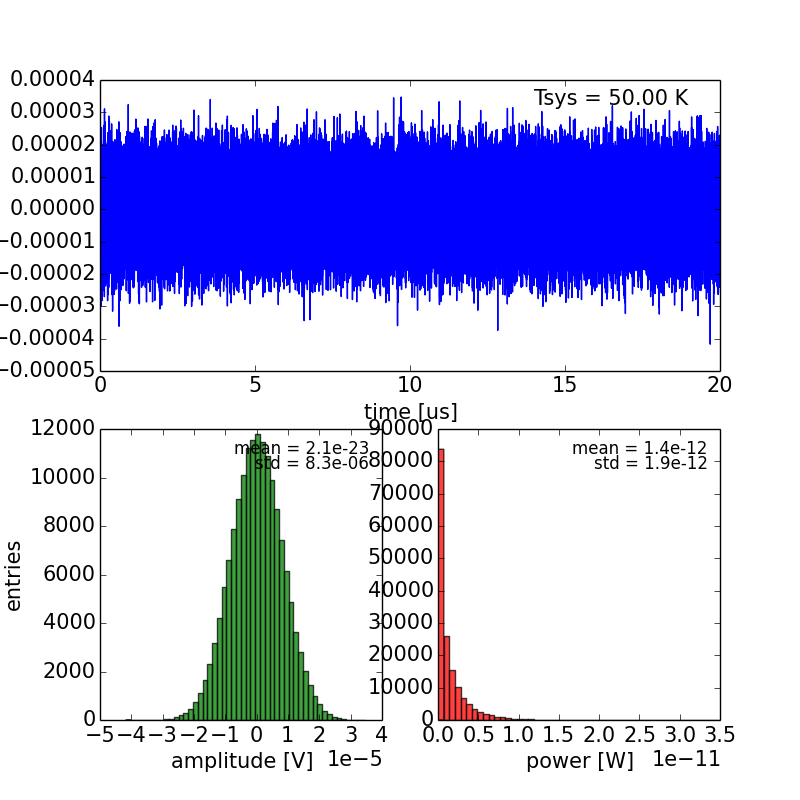
\includegraphics[width=0.49\linewidth]{noise.png}}
  \subfigure{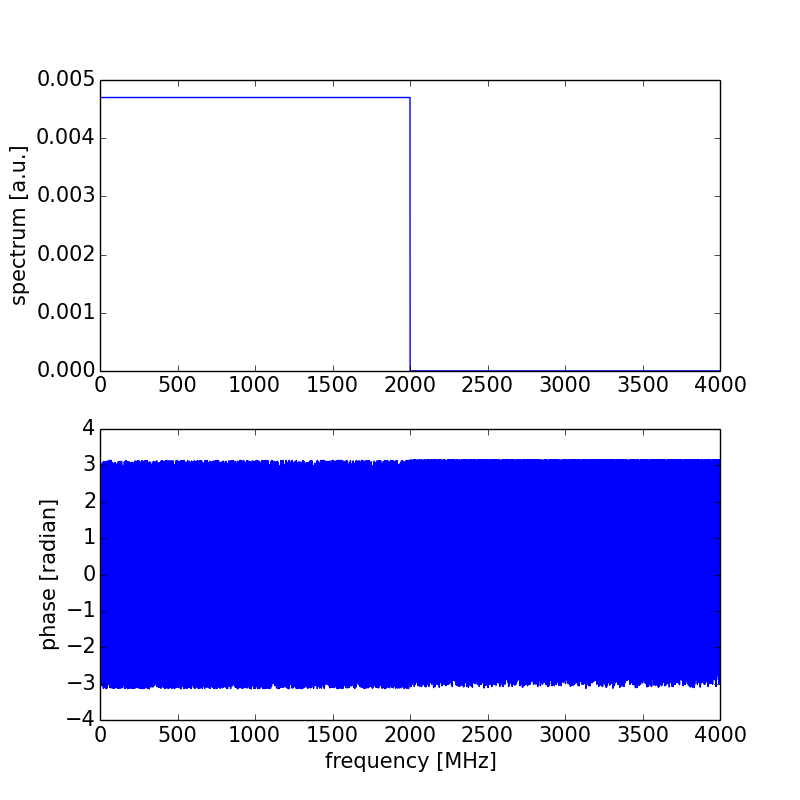
\includegraphics[width=0.49\linewidth]{specphasenoise.png}}
  \caption{Left: top:  waveform, bottom left:  amplitude distribution,
    bottom  right power  distribution. Right:  top:  spectrum, bottom:
    phase}
  \label{fig:flatspec}
\end{figure}


\begin{figure}[!ht]
  \centering
  \hspace*{-3ex}
  \subfigure{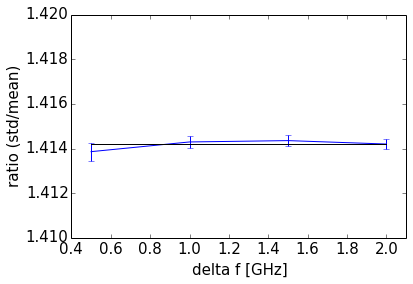
\includegraphics[width=0.49\linewidth]{ratiodiffBW.png}}
  \subfigure{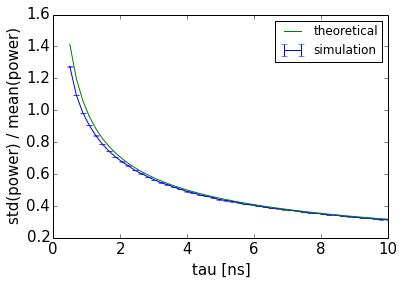
\includegraphics[width=0.49\linewidth]{rationumfilter.png}}
  \caption{left: ratio $\frac{\sigma}{\mu}$ versus the lower frequency
    $f_min$ of the noise spectrum. rigt: the ratio when we apply a low
    pass filter of frequency cut $f_{cut}= 1/\tau$ to the power. It is
    shown for three different $f_{min}$}
  \label{fig:bwfilt}
\end{figure}

\paragraph{numerical filter}
Now we  filter the  waveform (  after converting it  to power)  with a
numerical filter  (we set  the fft coefficient  to 0 for  the filtered
frequencies.).  The orignal waveform is issued from a spectrum between
0    and   2GHz.    We    show   in    fig.~\ref{fig:bwfilt}   (right)
$\frac{\sigma}{\mu}$  the ratio  for different  frequency cuts  of the
filter  where   the  x-axis  is  the   time  constant  $   \rm  tau  =
\frac{1}{f_{cut}}$.   We see that  it follows  very well  the expected
formula.\\ Now if  we vary the bandwidth and then  apply the filter we
obtain the result in the  fig.~\ref{fig:bwfilt2} (left).  We see now a
discrepancy between the expected ratio  and the simulated one.  We see
that if we reduce the bandwidth,  the ratio is lower than expected and
plateaus at  for the high  frequency filters (low $\tau$)  but matches
the formulas at  the low frequency filter (high  $\tau$).  This can be
understood  when  we  think  about  the  FFTs  (or  look  at  them  on
figure~\ref{fig:bwfilt2}).  The  fourier transform of the  power for a
signal at  frequencies in [f1  - f2] has  a contribution between  [0 ;
  $\Delta  B/2$], where  $\Delta B  = f2-f1$  and another  one between
[2*f1 ; 2*f2].  On the figure we see an example for an amplitude input
spectrum of  [1.5 ; 2  GHz].  If we  filter the power spectrum  with a
frequency  $f_{cut} $smaller  than  $\Delta B/2$  then  we follow  the
equation because  we have a full  or a continuous bandwidth  from [0 ;
  $f_{cut}$], if $f_{cut}$  is larger then we go into  the hole in the
power spectrum and  we don't add any frequency  in the average, that's
why the ratio goes to a constant.

\begin{figure}[!ht]
  \centering
  \hspace*{-3ex}
  \subfigure{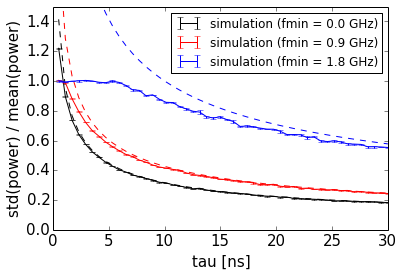
\includegraphics[width=0.49\linewidth]{rationumfilterdiffBW.png}}
  \subfigure{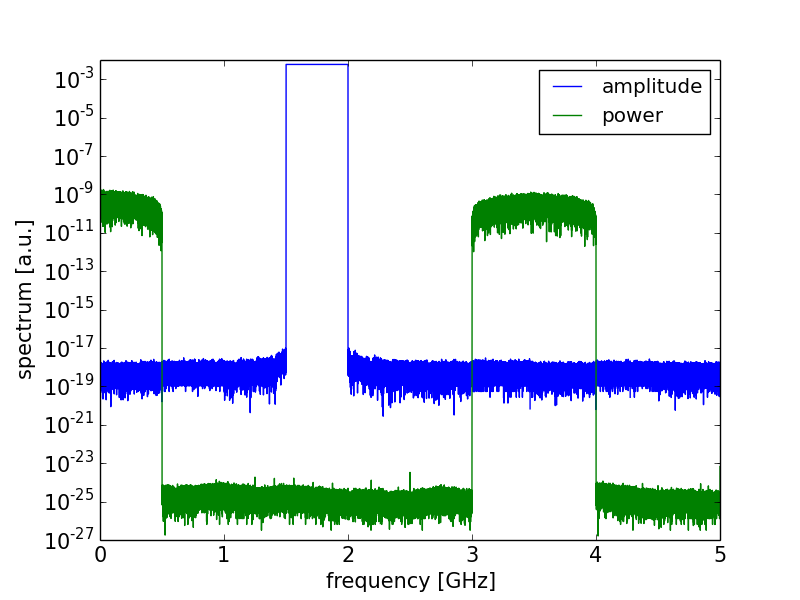
\includegraphics[width=0.49\linewidth]{specnoise.png}}
  \caption{left: ratio $\frac{\sigma}{\mu}$ versus the lower frequency
    $f_min$ of the noise spectrum. rigt: the ratio when we apply a low
    pass filter of frequency cut $f_{cut}= 1/\tau$ to the power. It is
    shown for three different $f_{min}$}
  \label{fig:bwfilt2}
\end{figure}

\paragraph{sliding window}
In  this paragraph,  instead  of filtering  by  cutting the  frequency
spectrum  we average over  several time  bins, i.e.  we use  a sliding
window  average.  If  we consider  $\tau$ as  the window  size  we see
(fig~\ref{fig:slidingwindow})  that  the   ratio  doesn't  follow  the
equation~\ref{eq:sigmamu}.  There is an additional factor to be added.
\begin{figure}[!ht]
  \centering
  \hspace*{-3ex}
  \subfigure{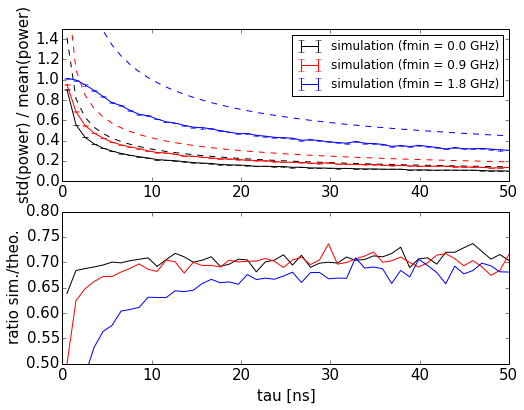
\includegraphics[width=0.60\linewidth]{slidingwindow.png}}
  \caption{$\frac{\sigma}{\mu}$ ratio after  applying a sliding window
    of size $\tau$ for different $f_{min}$}
  \label{fig:slidingwindow}
\end{figure}

We showed that the formula~\ref{eq:sigmamu}  can not be always used in
this  form. Some  conditions have  to  be matched  and the  processing
technique  (filtering  or other  sort  of  averaging)  can change  the
ratio.\\ It  can still  be used  as a figure  of merit  but it  is not
anymore representative  of the minimum  detectable signal (or  the one
sigma deviation from the mean).

\subsection{realistic spectrum}
Our detectors  have not  a flat spectrum  (cf fig.~\ref{fig:spectra}).
We first show  how we simulate it  and then we see how  to account for
this in the equation~\ref{eq:sigmamu}.

\paragraph{detectors gain}
The spectrum  that we need to  simulate our signal is  the spectrum at
the  input of  the power  detector. We  show here  that  this spectrum
depends only  on the antenna  and LNB gain.  \\ What comes out  of the
antenna + LNB is:
\begin{equation}
   \rm P(\nu) = \frac{1}{2}\int_\Omega F(\nu) A_{eff}(\nu) G_{LNB}(\nu)d\Omega
\end{equation}
with
\begin{equation}
  \rm F(\nu) = \frac{2k_B T \nu^2}{c^2}
\end{equation}
and

\begin{equation}
  \rm A_{eff}(\nu) = \frac{ G_{ant}(\nu)c^2 }{4\pi \nu^2 }
\end{equation}


So the  $\rm \nu^2$ cancels  out and we  have only:
\begin{equation}
   \rm P(\nu) = \frac{1}{4\pi}\int_\Omega k_B T G_{ant}(\nu) G_{LNB}(\nu) d\Omega= k_B T_{ant} G_{LNB}(\nu)
\end{equation}
Then the only dependence in frequency is given by the antenna gain and
the  amplifier gain.   For  the three  antenna  and LNB  that we  have
installed we have this data with:
\begin{itemize}
\item for EASIER antennas (DMX and GI301):spectrum measurement (in the field or at room temperature)
\item for GIGADuck antenna (Norsat) : IMEP measurement of the total gain antenna+LNB
\end{itemize}

\begin{figure}[!ht]
  \centering
  \hspace*{-3ex}
  \subfigure{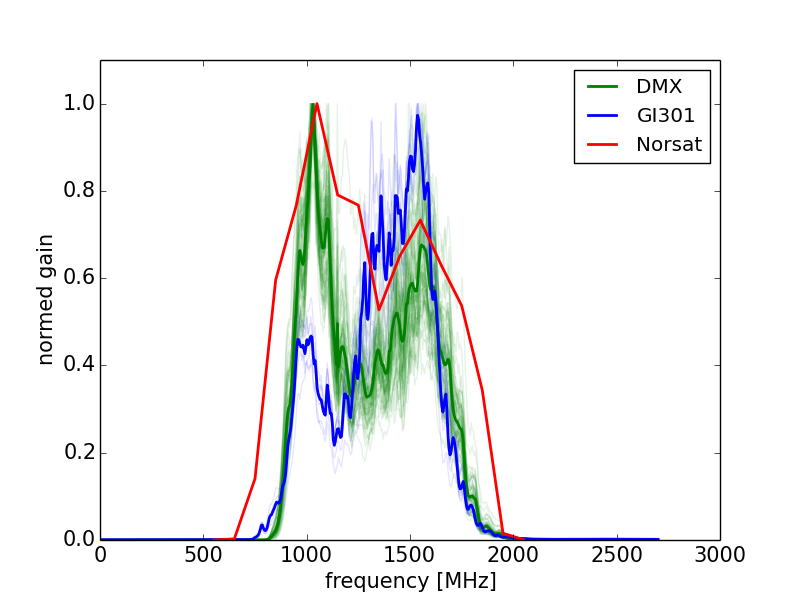
\includegraphics[width=0.60\linewidth]{spectra3.png}}
  \caption{gain spectra for the three types of LNB in the C-band.}
  \label{fig:spectra}
\end{figure}

\paragraph{simulation with realistic spectrum}
To simulate  a waveform with the  detector spectrum, we  set first the
fft with the  \textbf{square root of the power gain}  and the phase is
again drawn randomly from a uniform distribution between [$ \rm -\pi ;
  \pi$].
\paragraph{what is the bandwidth ?}
Now  we want  to know  how  to relate  the realistic  bandwith to  the
equation~\ref{eq:sigmamu}.  Usually  we take  the bandwith as  800 MHz
because of the definition of  the C-band (3.4-4.2 GHz). However we see
that the gain is not flat so what quantity should we take to enter the
equation~\ref{eq:sigmamu}  ?   One  can  think   about  the  following
definition:
\begin{equation}                                                                           
  \rm \Delta B = \frac{1}{G_{max}} \int G(\nu) \cdot d\nu  
  \label{eq:eqdeltab} 
\end{equation} 
This definition is usefull for instance to estimate the total power in
a band. For instance this  bandwidth will enter the calculation of the
average    power    (see    second    point    of    the    derivation
section\ref{sec:theory}) \\In  fact we  need to compute  the bandwidth
as:
\begin{equation}
  \rm \Delta B = \frac{1}{\sqrt{G_{max}}} \int \sqrt{G(\nu)} \cdot d\nu
  \label{eq:eqdeltabsqrt}
\end{equation}
To see this we can look  at the $\frac{\sigma}{\mu}$ ratio from a real
waveform of noise  coming from an antenna (a  DMX antenna) and compare
it with  the $\frac{\sigma}{\mu}$ ratio  of a flat  spectrum generated
waveform   with  $\Delta  B$   computed  as   eq~\ref{eq:eqdeltab}  or
eq~\ref{eq:eqdeltabsqrt}. (We need to apply a filter so that the ratio
is different from $\sqrt{2}$).
\begin{figure}[!ht]
  \centering
  \hspace*{-3ex}
  \subfigure{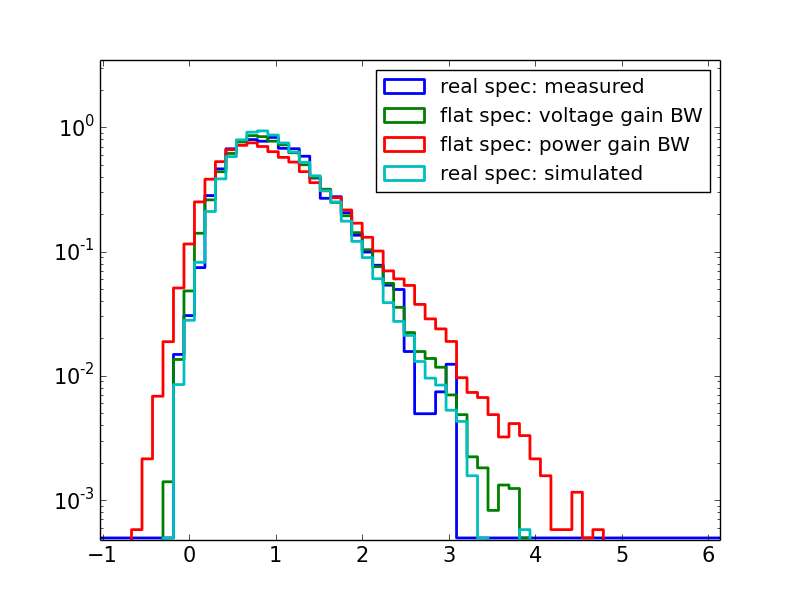
\includegraphics[width=0.60\linewidth]{noisedist.png}}
  \caption{noise distribution after power  filtering in 4 cases: blue:
    real waveform  from a DMX antenna. green:  flat spectrum generated
    waveform with bandwidth according eq~\ref{eq:eqdeltabsqrt}, red:flat
    spectrum    generated    waveform    with   bandwidth    according
    eq~\ref{eq:eqdeltab},  light  blue:   waveform  generated  from  the
    spectrum in fig~\ref{fig:spectra}}
  \label{fig:spectra}
\end{figure}
At the end the bandwidth are given is the table~\ref{tab:tabdeltab}.
\begin{table}[h!]
  \centering
  \caption{bandwidths}
  \label{tab:tabdeltab}
  \begin{tabular}{|c||c|c|c|}
    \hline
    antenna type & GI301  & DMX & Norsat \\
    \hline
    voltage bandwidth & 704 $\rm \pm 29$& 689 $\rm \pm$ 46 & 901\\
    \hline
    power bandwidth & 437 $\rm \pm 30$& 445 $\rm \pm$ 56 & 684\\
    \hline
  \end{tabular}
\end{table}







